Международные сайты исследователей содержат
большое число подготовленных структурированные данных. 
К сожалению, большинство из них представлены на китайском и английский языках. Для их адаптации
предложен подход, использующий большие языковые модели как средство перевода на русский язык.
В качестве открытого решения был выбран языковой ассистент llama3, показывающий 


Перевод 7500 задач выполнялся в течении 12 часов.
Полученные результаты приведены в предметном репозитории \footnote{\url{https://huggingface.co/datasets/NMashalov/olympiad_task_translation}}


\begin{figure}[h]
    \centering
    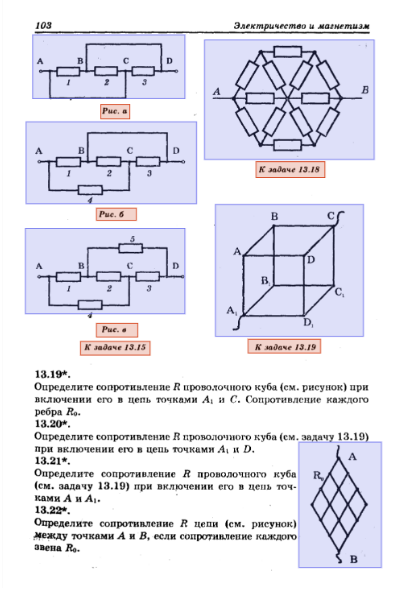
\includegraphics[width=0.5\textwidth]{assets/work/dataset/kirik_labeling.png}
    \caption{Пример аннотированной иллюстрации из книги Генденштейн, Кирик, Гельфгат: 1001 задача по физике}
    \label{annotation}
\end{figure}


Для адаптации корпуса задач также были подготовлены



